%************************************************
\chapter{Developer Guide}\label{ch:developer_guide} % $\mathbb{ZNR}$
%************************************************

This chapter will guide the reader through the different requirements and their implementation in the application.

Having finished with the requirements a section highlighting certain problems or special cases that were encountered during the development will be described.

\section{Implementation of the requirements}
\label{sec:implementation_requirements}

\subsection{Web-requirements}

Requirements \texttt{WR01}, \texttt{WR02} and \texttt{WR03} are implemented in the \texttt{PageHandler}-class:

It requests a provided \ac{URL} via its \texttt{FetchUrl()}-method that will return a \texttt{SimpleWebResponse}-object. The \texttt{SimpleWebResponse}-object encapsulates just a title, body and a url - all elements needed to display a web-page.

To fulfil requirement \texttt{WR04} it is necessary to assign a \texttt{WebResponse} after catching an exception that is thrown by the \texttt{.NET}-framework if a response does not contain a 200 (OK)-message:

\begin{lstlisting}[caption=Fetching \ac{URL}s with error-codes]
try
{
       this.Request = WebRequest.Create(this.RequestUrl);
       this.Response = this.Request.GetResponse();
}
catch (WebException e)
{
       logger.Error("WebException ({0}) occured when fetching the url: {1}", e.Message, this.RequestUrl);
       this.Response = e.Response;
}
\end{lstlisting}

\texttt{WR04} is implemented in the \texttt{PagePresenter}: the page-presenter starts a \texttt{FetchUrl()}-method-call via an asynchronous delegate and provides a callback-mechanism to its \texttt{Done()}-method.

\begin{lstlisting}[caption=Fetching \ac{URL}s with error-codes]
Func<SimpleWebResponse> method = pageHandler.FetchUrl;
method.BeginInvoke(Done, method);
\end{lstlisting}

When the \texttt{Done()}-method is invoked, the presenter calls the view's \texttt{DisplayWebpage()}-method that prints the received \ac{HTML}-code\footnote{See \autoref{sec:implementation_view} to see details for the necessary view-implementation.}.

\subsection{Homepage-Requirements}

The homepage is saved as a simple string. This leads to the possibility to save it via the \texttt{ApplicationSettings} - a facility provided by the \texttt{.NET} framework.

The only problem in this implementation is the fact that only the \texttt{WinForms} project is allowed to access the application-settings\footnote{It would be possible to provide a reference to the \ac{GUI}-project in the logic-project. However this would lead to a dependency between the logic-project and the \ac{GUI} - a circumstance that should be prevented by utilizing the \ac{MVP}-pattern. Due to this fact the \ac{GUI} writes the application settings and the logic stays independent from the \ac{GUI}.}.

Due to this reason the code to write the string is located in the \texttt{SettingsWindow}:

\begin{lstlisting}
private void SaveSettings(String homePage)
        {
            Settings settings = Settings.Default;
            settings.Homepage = homePage;
            settings.Save();
        }
\end{lstlisting}

\subsection{Favourite-requirements}

The requirements \texttt{FR01} and \texttt{FR02} were implemented in the \texttt{Favourite} and \texttt{FavouriteHandler}-classes.

Apart from handling the adding (\texttt{AddEntry()}), deleting (\texttt{DeleteFavourite()}) and editing (\texttt{EditFavourite()}) of favourites, the \texttt{FavouriteHandler} also handles the saving (\texttt{SaveFavourite()}) and loading (\texttt{LoadFavourites()}) of favourites.

Requirement \texttt{FR04} is fulfilled by the  \texttt{FavouritePresenter}: upon creation the presenter determines the file-path for the favourite file and sets it in the \texttt{FavouriteHandler}:

\begin{lstlisting}
private void SetUpHandler()
        {
            String appFolder = Environment.GetFolderPath(Environment.SpecialFolder.ApplicationData);
            String history = "Favourites.xml";
            this._FavouriteHandler.SetFilePath(Path.Combine(appFolder, history));
            this._FavouriteHandler.LoadFavourite();
        }
\end{lstlisting}

This approach was chosen to keep the \texttt{FavouriteHandler} reusable, whereas the presenter can be considered application-specific.

Requirement \texttt{FR03} was implemented in the \ac{GUI}: when the user clicks an element in the favourite-list, the element is determined and the url of the favourite is written into the \ac{URL}-text-field. After this has happened, a standard \ac{URL}-request is issued and the \ac{URL} will be displayed in the active tab.

\subsection{History-requirements}

The implementation of the history-requirements is similar to the those of the favourites.

The main-classes are \texttt{History} and \texttt{HistoryHandler}, whereas the loading on start-up is provided by the \texttt{HistoryPresenter}.

\begin{lstlisting}
private void SetUpHandler()
        {
            String appFolder = Environment.GetFolderPath(Environment.SpecialFolder.ApplicationData);
            String history = "History.xml";
            this._HistoryHandler.SetFilePath(Path.Combine(appFolder, history));
            this._HistoryHandler.LoadHistory();
        }
\end{lstlisting}

The loading of a \ac{URL} on user-interaction is implemented in the \ac{GUI} via a \texttt{NodeMouseClick-Event} on the \texttt{History-TreeView}.

\subsection{Printing-requirements}

Requirement \texttt{PR01} was implemented in the \texttt{MainWindow} and the \texttt{PrintPresenter}-classes.

The \texttt{PrintPresenter}'s \texttt{Print()}-method will be called for every page that needs to be printed.

The method will determine the size of the String that shall be printed and set the \texttt{HasMorePages}-property to true if the String would not fit onto one page:

\begin{lstlisting}
public void Print(System.Drawing.Printing.PrintPageEventArgs e)
        {
            
            Font font = _PrintView.CurrentFont;
            int charactersOnPage = 0;
            int linesPerPage = 0;

            // Sets the value of charactersOnPage to the number of characters 
            // of PrintString that will fit within the bounds of the page.
            e.Graphics.MeasureString(PrintString, font,
                e.MarginBounds.Size, StringFormat.GenericTypographic,
                out charactersOnPage, out linesPerPage);

            // Draws the string within the bounds of the page
            e.Graphics.DrawString(PrintString, font, Brushes.Black,
                e.MarginBounds, StringFormat.GenericTypographic);

            // Remove the portion of the string that has been printed.
            PrintString = PrintString.Substring(charactersOnPage);

            // Check to see if more pages are to be printed.
            e.HasMorePages = (PrintString.Length > 0);
        }
\end{lstlisting}

\subsection{User-interface requirements}

All actions can be performed via a \ac{GUI}: see \autoref{ch:user_guide} for an introduction of how to use the provided \ac{GUI}.

As the \ac{GUI} was implemented via the \texttt{WinForms} designer and all actions that are not just altering the \ac{GUI} are passed to the presenters, no significant logic that has not already been mentioned is implemented in the \ac{GUI}.

Due to this fact no more implementation-details about the requirements \texttt{GR01} and \texttt{GR02} will be described.

\section{Details of the implementation}
\label{sec:details_implementation}

Apart from just providing an overview over the requirements and their corresponding implementation, this section will provide an overview over certain areas of code that might be hard to understand without further explanation, but are not directly linked to a certain requirement.

\subsection{View}

All \ac{GUI} classes have a common ancestor: the class \texttt{ThreadingView}:

\begin{figure}[H]
\begin{center}
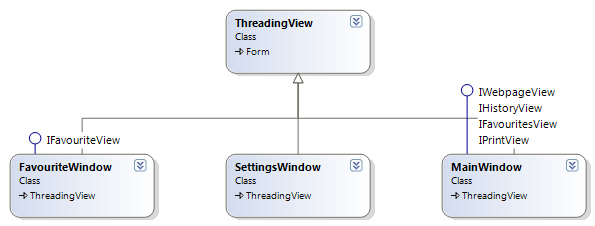
\includegraphics[width=\textwidth]{gfx/view_diagram.png}
\caption{\ac{GUI} class hierarchy}
\label{fig:view_diagram}
\end{center}
\end{figure}

Due to this approach all classes are able to use the \texttt{UpdateUI()}-method of this class when another thread wants to alter a \ac{GUI}-control:

\begin{lstlisting}
protected void UpdateUI(MethodInvoker uiDelegate)
        {
            if (InvokeRequired)
            {
                this.Invoke(uiDelegate);
            }
            else
            {
                uiDelegate();
            }
        }
\end{lstlisting}

This is necessary as only the thread that created a \ac{GUI}-component is allowed to update it.
Via \texttt{InvokeRequired} it is possible to check if another thread tries to modify the component (returns \texttt{true} if another thread wants to modify it, \texttt{false} otherwise).

In the current application this behaviour might occur when the page-request-thread calls the \texttt{PagePresenter's} \texttt{done()} method and the presenter tries to force the view to display the web-page.
To prevent an exception from ocurring the code to update the \ac{GUI}-component is called like this:

\begin{lstlisting}
public void DisplayWebPage(SimpleWebResponse response)
        {
            foreach (TabPage page in this.webSitesTabControl.TabPages)
            {
                if (page.Name.Equals(response.Url))
                {
                    MethodInvoker uiDelegate = delegate
                    {
                        page.Controls[0].Text = response.Html;
                        page.Text = response.Title;
                    };
                    UpdateUI(uiDelegate);
                }
            }
        }
\end{lstlisting}

This way the \ac{GUI}-thread will alter the component.

\subsection{Observer-pattern}

As already mentioned in \autoref{subsec:separate_change} the observer pattern is used to keep the different presenter up-to-date.
Namely this approach concerns the \texttt{Favourite-} and \texttt{HistoryHandlers} and their respective presenters.

However the implementation was not performed utilizing multiple classes as described in \textcite{gamma1994}, but by utilizing \texttt{.NET} specific concepts like delegates.

Therefore the handlers declare a delegate that the observers can use.
Moreover an event is declared that will chain the multiple methods of the observers so that every observer will be notified of the changes.
These subscribed methods will then be called, as soon as a notification-worthy event occurs.

% TODO Fancy overview.

\subsection{Singleton-pattern}



\subsection{Serialisation}

